% !TEX root = ./notes.tex
\chapter[Stellar Atmospheres]{Stellar Atmospheres}

In the atmosphere of the star, the optical depth approaches unity, and we can no longer treat the radiation field as being isotropic. Let's consider the time-independent problem ($\partial_{t}\to 0$) of a plane-parallel atmosphere. Define the \emph{optical depth} via the equation
\begin{equation}\label{e.optical-depth}
\tau_{\nu} = - \int _{z}^{\infty}\!\rho\kappa_{\nu}\,\dif z'.
\end{equation}
We've introduced the minus sign to account for the fact that $\tau_{\nu}$ increases with decreasing $z$.
Changing variables from $r$ to $\tau_{\nu}$, and defining $\mu = \unitk\cdot\unitn$, where \unitn\ is the direction along the ray, gives
\begin{equation}\label{e.planar}
\mu\frac{\partial I_{\nu}}{\partial\tau_{\nu}} = I_{\nu}-S_{\nu},
\end{equation}
where 
\begin{equation}\label{e.source}
S_{\nu} \equiv \frac{1}{\kappa_{\nu}}\left(\frac{\varepsilon_{\nu}}{4\pi} + \kappa_{\nu}^{\mathrm{sca}}J_{\nu}\right)
\end{equation}
is the \emph{source function}. In LTE, we can write $S_{\nu} = (1-A_{\nu})B_{\nu} + A_{\nu}J_{\nu}$, where $A_{\nu} \equiv \kappa_{\nu}^{\mathrm{sca}}/\kappa_{\nu}$ is the \emph{albedo}.  Recall that $J_{\nu} = (4\pi)^{-1}\int\dif\Omega\,I_{\nu}$ is the angle-average of $I_{\nu}$.

\section{The Eddington Approximation}

We noted that in thermal equilibrium, $P_{\nu} = c^{-1}\int_{-1}^{1}\dif\mu\,\mu^{2}I_{\nu} = u_{\nu}/3$. This holds even when the radiation is not thermal, so long as it is isotropic to terms linear in $\mu$.  To make this concrete, suppose we write
\[ I_{\nu}(\mu) = I_{\nu}^{(0)} + \mu I_{\nu}^{(1)} + \mu^{2}I_{\nu}^{(2)} + \ldots. \]
Here we are assuming that terms marked $(0)$ are much larger than terms marked $(1)$, etc.  To lowest order, the energy density, flux, and momentum flux are then
\begin{eqnarray*}
u_{\nu} &=& \frac{2\pi}{c}\int_{-1}^{1}\dif\mu\,I_{\nu}(\mu) = \frac{4\pi}{c} I_{\nu}^{(0)},\\
F_{\nu} &=& 2\pi\int_{-1}^{1}\dif\mu\,\mu\,I_{\nu}(\mu) = \frac{4\pi}{3} I_{\nu}^{(1)},\\
P_{\nu} &=& \frac{2\pi}{c}\int_{-1}^{1}\dif\mu\,\mu^{2}\,I_{\nu}(\mu) = \frac{4\pi}{3c}I_{\nu}^{(0)} = \frac{u_{\nu}}{3}.
\end{eqnarray*}
The \emph{Eddington approximation} then consists of treating the radiation field as if its anisotropy is linear in $\mu$ \emph{everywhere}, so that the above relations hold; in particular, it means assuming that $P_{\nu} = u_{\nu}/3$ everywhere.

\section[Grey Atmosphere]{A Grey Atmosphere}

Finally, to get an analytical approximation to the structure of the solar atmosphere, let's consider a grey atmosphere in LTE, i. e., one for which $\kappa_{\nu}^{\mathrm{abs}} = \kappa^{\mathrm{abs}}$ and $\kappa_{\nu}^{\mathrm{sca}} = \kappa^{\mathrm{sca}}$ are independent of frequency. Equation~(\ref{e.planar}) can then be integrated over all frequencies to become
\begin{equation}\label{e.J-grey}
\mu\frac{\partial I}{\partial\tau} = I-S.
\end{equation}
Integrating over all angles (note that we can pull the derivative wrt $\tau$ out of the integral) gives
\begin{equation}\label{e.H-grey}
\frac{1}{4\pi}\frac{\partial F}{\partial\tau} = J - S = 0.
\end{equation}
Why does the right-hand side vanish? Note that $S-J = (1-A)(B-J)$.  Clearly $S = J$ if $A = 1$ (a pure scattering atmosphere).  If $A \ne 1$, so that there is some absorption, then the condition of detailed balance, equation~(\ref{e.detail-balance}), implies that $\varepsilon_{\nu} = 4\pi\kappa^{\mathrm{abs}}B_{\nu}(T)$; inserting this into equation~(\ref{e.rad-equil}), factoring out the constant $\kappa^{\mathrm{abs}}$, and integrating over $\nu$ implies that $B - J = 0$, and hence $S - J = 0$. Note that $J = B$ does \emph{not} necessarily imply that $I_{\nu} = B_{\nu}$!

To make use of the Eddington approximation, first multiply equation~(\ref{e.J-grey}) by $\mu$ and integrate over $2\pi\,\dif\mu$ to obtain
\begin{equation}\label{e.K-grey}
c\frac{\partial P}{\partial\tau} = F,
\end{equation}
the integral over $\mu S$ vanishing because it is odd in $\mu$. Equation~(\ref{e.H-grey}) implies that $F$ is constant; hence we can integrate equation~(\ref{e.K-grey}) at once to obtain
\begin{equation}\label{e.KH}
cP = F(\tau + \tau_{0}),
\end{equation}
where $\tau_{0}$ is a constant of integration.

We are now ready to apply the Eddington approximation.  We take $P = u/3 = 4\pi J/(3c)$ and insert it into equation~(\ref{e.KH}) to obtain $4\pi J = 3F(\tau + \tau_{0})$. Since $J = S$, equation~(\ref{e.J-grey}) becomes
\begin{equation}
\mu\frac{\partial I}{\partial\tau} = I - \frac{3}{4\pi}F(\tau+\tau_{0}).
\end{equation}
This first-order differential equation (recall $F$ is constant) is now solvable,
\begin{eqnarray}
I(\mu,\tau=0) &=& \frac{1}{\mu}\int_{0}^{\infty}\!\frac{3}{4\pi}F(\tau + \tau_{0}) e^{-\tau/\mu}\,\dif\tau,\nonumber\\
  &=& \frac{3}{4\pi}F(\mu + \tau_{0}).
\end{eqnarray}
Now at $\tau = 0$, all of the flux must be outward-directed ($\mu >0$), so $I(\mu < 0,\tau = 0) = 0$ if the star is not irradiated by another source.  Note that the Eddington approximation is clearly violated here.  Still, we will see later that this approximation is not too terrible. 

To determine $\tau_{0}$, multiply $I(\mu,\tau = 0)$ by $\mu$ and integrate over all angles,
\begin{equation}
F = 2\pi\int_{0}^{1}\!\mu I(\mu,0)\,\dif\mu = \frac{1}{2}\int_{0}^{1}\!3F(\mu + \tau_{0})\,\mu\,\dif\mu = F\left(\frac{1}{2} + \frac{3}{4}\tau_{0}\right);
\end{equation}
Hence $\tau_{0} = 2/3$. Now, since we are in LTE, $P = aT^{4}/3$. Further, let us define an effective temperature by the relation $F = \sigma_{\mathrm{SB}}T_{\mathrm{eff}}^{4}$.  Substituting these definitions and the value of $\tau_{0}$ into equation~(\ref{e.KH}) gives us the atmospheric temperature structure,
\begin{equation}\label{e.Eddington}
T^{4}(\tau) = \frac{3}{4}T_{\mathrm{eff}}^{4}\left(\tau + \frac{2}{3}\right).
\end{equation}
Thus $T(\tau  = 0) = 2^{-1/4} T_{\mathrm{eff}}$ and $T(\tau = 2/3) = T_{\mathrm{eff}}$.  To get the spectral distribution, go back to equation~(\ref{e.planar}) and (assuming the atmosphere has some absorption so that the matter and radiation can come into equilibrium) insert $S_{\nu} = B_{\nu}(T)$; solving for $I_{\nu}$ at $\tau = 0$ then gives
\begin{equation}\label{e.spectral}
I_{\nu}(\mu,\tau=0) = \frac{1}{\mu}\int_{0}^{\infty}\!B_{\nu}\left[T(\tau)\right] \, e^{-\tau/\mu}\,\dif\tau.
\end{equation}
A plot of the spectral distribution for the emergent flux is shown (\emph{open circles}) in Fig.~\ref{f.spectral}. For comparison, a plot of the Planck distribution (\emph{solid line}) is also shown. Both fluxes are normalized to the total flux.

\begin{figure}[htbp]
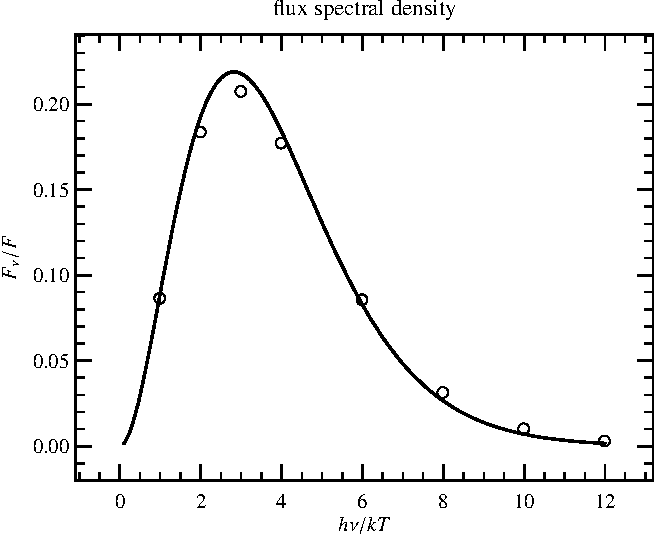
\includegraphics[width=4in]{plots_out/spectral_distribution}
\caption{\label{f.spectral} Spectral distribution from a grey atmosphere. The open circles are from Chandrasekhar, \emph{Radiative Transfer}; the solid line is the Planck distribution.}
\end{figure}

\section{A Constant-Flux Atmosphere}

Consider an atmosphere (planar geometry) with constant gravity $\bvec{g} = -g \bvec{e}_{r}$ and a constant outward-directed flux $\bvec{F} = F\bvec{e}_{r}$. Let's assume that the gas can be described as a mixture of an ideal gas and radiation.  Further assume that the opacity is constant and grey (i.e., Thomson) and that the atmosphere is in LTE.

Under what conditions does the gas pressure dominate?
\begin{eqnarray}
\Pgas&\gg& \Prad\nonumber\\
\frac{\rho kT}{\mu \mb} &\gg& \frac{1}{3}aT^{4}\nonumber\\
\rho &\gg& 0.03\mu \left(\frac{T}{10^{7}\nsp\K}\right)^{3}\nsp\grampercc.
\end{eqnarray}
Note the magnitude; this is easily satisfied for stars like the sun.  Now consider the equation for the flux,
\begin{equation}
F = -\frac{1}{3}\frac{ac}{\rho\kappa}\frac{\dif T^{4}}{\dif r}.
\end{equation}
Let's rewrite this using the identity $\dif/\dif r = (\dif P/\dif r)(\dif/\dif P) = -\rho g (\dif/\dif P)$ as
\begin{equation}\label{e.F}
F = -\frac{c}{\rho\kappa}\frac{\dif \Prad}{\dif r} = \frac{cg}{\kappa}\frac{\dif \Prad}{\dif P}.
\end{equation}
It is critical to remember that $P$ is the \emph{total} pressure, $P = \Prad + \Pgas$. Now for something clever.  Since $F = L/(4\pi R^{2})$ and $g = GM/R^{2}$, we can cancel $R^{2}$ from both sides of equation~(\ref{e.F}). Further, recall that $4\pi GMc/\kappa = \Ledd$, the Eddington luminosity, so that we can write
\begin{equation}\label{e.Prad}
\frac{\dif \Prad}{\dif P} = \frac{L}{\Ledd}.
\end{equation}
Since $\dif \Prad/\dif P = 4 (\Prad/T) (\dif T/\dif P)$, we can work out immediately how $\dif T/\dif P$ changes with depth.

Since we are assuming an atmosphere with constant $L/\Ledd$, we can integrate equation~(\ref{e.Prad}) inward from the photosphere,
\begin{equation}
\Prad - P_{\mathrm{rad,0}} = \frac{L}{\Ledd}(P-P_{0}).
\end{equation}
Later on we will get the correct expression for the photospheric values (with subscript ``0''), but for now, let's go sufficiently deep that we can ignore the outer boundary, in which case,
\begin{equation}
\Prad \approx \frac{L}{\Ledd}P = \frac{L}{\Ledd}(\Pgas + \Prad).
\end{equation}
Dividing through by \Pgas, we obtain the desired result,
\begin{equation}
\frac{\Prad}{\Pgas} = \frac{L}{\Ledd}\left(1-\frac{L}{\Ledd}\right)^{-1}.
\end{equation}
The right-hand side is a constant; note that for the sun, $L/\Ledd \approx  3\times 10^{-5}$.

\section{The Curve of Growth}

A classical technique in the analysis of stellar spectra is to construct the \emph{curve of growth}, which relates the equivalent width of a line $W_{\nu}$ to the opacity in the line. This discussion follows Mihalas, \emph{Stellar Atmospheres}.

Let's first get the opacity in the line.  We saw in class that the cross-section for the transition $i\to j$ could be written as 
\begin{equation}\label{e.cross-section}
\sigma_{\nu} = \left(\frac{\pi e^{2}}{m_{e}c}\right)f_{ij}\phi_{\nu},
\end{equation}
where the first term is the classical oscillator cross-section, $f_{ij}$ is the oscillator strength and contains the quantum mechanical details of the interaction, $\phi_{\nu}$ is the line profile.  Now recall that the opacity is given by $\kappa_{\nu} = n_{i}\sigma_{\nu}/\rho$, where $n_{i}$ denotes the number density of available atoms in state $i$ available to absorb a photon.  Furthermore, we need to allow for \emph{stimulated emission} from state $j$ to state $i$. With this added, the opacity is (I'm writing it as $\chi_{\nu}$ to distinguish it from the \emph{continuum opacity})
\begin{equation}\label{e.opacity}
\rho\chi_{\nu} = \left(\frac{\pi e^{2}}{m_{e}c}\right)f_{ij}\phi_{\nu}n_{i}\left[1 - \frac{g_{i}}{g_{j}}\frac{n_{j}}{n_{i}}\right].
\end{equation}
If we are in LTE, then the relative population of $n_{i}$ and $n_{j}$ follow a Boltzmann distribution,
\[ 1 - \frac{g_{i}}{g_{j}}\frac{n_{j}}{n_{i}} = 1- \exp\left(-\frac{h\nu}{kT}\right). \]
This ensures we have a positive opacity. If our population were inverted, i.~e., more atoms in the upper state $j$, then the opacity would be negative and we would have a \emph{laser}.

Now for the line profile.  In the case where we have doppler broadening and damping, the profile follows the \emph{Voigt} function,
\begin{equation}\label{e.voigt} \phi_{\nu} = \frac{1}{\Delta \nu_{D}}H(a,v), \end{equation}
where $\Delta\nu_{D} \equiv \nu u_{0}/c$ is the doppler width, with $u_{0}$ being the mean (thermal) velocity of the atoms, $a \equiv \Gamma/(4\pi\Delta\nu_{D})$ is the ratio of the damping width $\Gamma$ to the doppler width, and $v \equiv \Delta\nu/\Delta\nu_{0}$ is the difference in frequency from the line center in units of the doppler width.

Let's combine the line opacity with the continuum opacity and solve the equation of transfer.
For simplicity, we are going to assume pure absorption in both the continuum and the line.  Under these conditions, the source function is (see the notes on the Eddington atmosphere) $S_{\nu} = B_{\nu}$, the Planck function. For a plane-parallel atmosphere, the equation of transfer is then
\begin{equation}\label{e.cg-transfer}
\mu\frac{\dif I}{\dif\tau} = I_{\nu} - B_{\nu}
\end{equation}
where $\mu$ is the cosine of the angle of the ray with vertical. Solving equation~(\ref{e.cg-transfer}) for the emergent intensity at $\tau_{\nu} = 0$ gives
\begin{equation}\label{e.intensity}
I_{\nu}(\mu) = \frac{1}{\mu}\int_{0}^{\infty}\!B_{\nu}[T(\tau_{\nu})] \exp(-\tau_{\nu}/\mu) \,\dif\tau_{\nu}.
\end{equation}
The opacity is given by
\begin{equation}\label{e.total-opacity}
\kappa_{\nu} = \kappa_{\nu}^{C} + \chi_{\nu},
\end{equation}
where $\kappa_{\nu}^{C}$ is the continuum opacity and $\chi_{\nu} = \chi_{0}\phi_{\nu}$ is the line opacity, with 
\[
\chi_{0} = \frac{1}{\rho}\left(\frac{\pi e^{2}}{m_{e}c}\right)f_{ij}n_{i}\left(1 - e^{h\nu_{\ell}/kT}\right)
\]
being the line opacity at the line center $\nu_{\ell}$. 

As a further simplification, we can usually ignore the variation with $\nu$ in $\kappa_{\nu}^{C}$ over the width of the line. As a more suspect approximation (although it is not so bad in practice), let's assume that $\beta_{\nu} \equiv \chi_{\nu}/\kappa_{C}$ is independent of $\tau$. With this assumption we can write $\dif\tau_{\nu} = (1+\beta_{\nu})\dif\tau$, where $\tau = -\rho\kappa^{C}\,\dif z$. Finally, let's assume that in the line forming region, the temperature does not vary too much, so that we can expand $B_{\nu}$ to first order in $\tau$,
\[ B_{\nu}[T(\tau)] \approx B_{0} + B_{1}\tau, \]
where $B_{0}$ and $B_{1}$ are constants.
Inserting these approximations into equation~(\ref{e.intensity}), multiplying by the direction cosine $\mu$ and integrating over outward bound rays gives us the flux,
\begin{eqnarray}\label{e.flux}
F_{\nu} &=& 2\pi\int_{0}^{1}\!\int_{0}^{\infty}\!\left[B_{0}+B_{1}\tau\right]\exp\left[-\frac{\tau}{\mu}(1+\beta_{\nu})\right] \left(1+\beta_{\nu}\right) \,\dif\tau\,\dif\mu\nonumber\\
 &=& \pi\left[ B_{0} + \frac{2}{3}\frac{B_{1}}{1+\beta_{\nu}}\right].
\end{eqnarray}
Far from the line-center, $\beta_{\nu}\to 0$, implying that the continuum flux is
\[ F_{\nu}^{C} = \pi\left[B_{0} + \frac{2B_{1}}{3}\right]. \]
Hence the depth of the line is
\begin{equation}\label{e.line-depth}
A_{\nu} \equiv 1 - \frac{F_{\nu}}{F_{\nu}^{C}} = A_{0}\frac{\beta_{\nu}}{1+\beta_{\nu}},
\end{equation}
where
\begin{equation}\label{e.A0-curve-growth}
 A_{0} \equiv \frac{2B_{1}/3}{B_{0} + 2B_{1}/3}
 \end{equation}
is the depth of an infinitely opaque ($\beta_{\nu}\to\infty$) line. 

\noindent Now that we have the depth of the line $A_{\nu}$ we can compute the \emph{equivalent width},
\begin{equation}\label{e.W}
W_{\nu} \equiv \int_{0}^{\infty}\! A_{\nu}\,\dif\nu = A_{0}\int_{0}^{\infty}\!\frac{\beta_{\nu}}{1+\beta_{\nu}}\,\dif\nu.
\end{equation}
Let's change variables from $\nu$ to $v = \Delta\nu/\Delta\nu_{D} = (\nu-\nu_{\ell})/\Delta\nu_{D}$.  Since $H(a,v)$ is symmetrical about the line center, we will just integrate over $\Delta\nu >0$, giving
\begin{equation}\label{e.Wv}
 W_{\nu} = 2A_{0}\Delta\nu_{D}\int_{0}^{\infty}\!\frac{\beta_{0}H(a,v)}{1+\beta_{0}H(a,v)}\,\dif v,
 \end{equation}
with $\beta_{0} = \chi_{0}/(\kappa^{C}\Delta\nu_{D})$.

It's useful to understand the behavior of $W_{\nu}$ in various limits.  
First, at small line optical depth ($\beta_{0}\ll 1$) only the core of the line will be visible. Recall that in the core of the line, $H(a,v) \approx \exp(-v^{2})$ so we insert this into equation~(\ref{e.Wv}) and expand the denominator to give
\begin{eqnarray}\label{e.linear}
W_{\nu}^{\star} \equiv \frac{W{\nu}}{2A_{0}\Delta\nu_{D}} &=& \int_{0}^{\infty} \!\sum_{k=1}^{\infty}(-1)^{k-1}\beta_{0}^{k}e^{-kv^{2}}\,\dif v\nonumber\\
 &=& \frac{1}{2}\sqrt{\pi}\beta_{0}\left[1-\frac{\beta_{0}}{\sqrt{2}} + \frac{\beta_{0}^{2}}{\sqrt{3}} - \ldots\right].
\end{eqnarray}
Here $W_{\nu}^{\star}$ is the \emph{reduced equivalent width}.
Notice that since $\beta_{0}\propto 1/\Delta\nu_{D}$ (cf.~eq.~[\ref{e.voigt}]), the equivalent width $W_{\nu}$ is independent of $\Delta\nu_{D}$ in this \emph{linear regime}.
Physically, in the limit of small optical depth, each atom in state $i$ is able to absorb photons, and the flux removed  is just proportional to the number of atoms $n_{i}$.

As we increase $\beta_{0}$ eventually the core of the line saturates---no more absorption in the core is possible.  As a result, the equivalent width should be nearly constant until there are so many absorbers that the damping wings contribute to the removal of flux.  In the \emph{saturation regime}, the Voigt function is still given by $e^{-v^{2}}$, but we can no longer assume $\beta_{0}\ll 1$, so our expansion in equation~(\ref{e.linear}) won't work. Let's go back to our integral, eq.~(\ref{e.Wv}), change variables to $z= v^{2}$, and define $\alpha = \ln\beta_{0}$ to find
\[
W_{\nu}^{\star} = \frac{1}{2}\int_{0}^{\infty}\!\frac{z^{-1/2}}{e^{z-\alpha}+1}\,\dif z.
\]
This may not look like an improvement, but you might notice that it bears a resemblance to a Fermi-Dirac integral (see the notes on the equation of state). That means that very smart people figured out tricks to handle these integrals and all we have to do is look up what they did.  In this case we have Sommerfeld to thank. In this saturation regime,
\begin{equation}\label{e.saturation}
W_{\nu}^{\star} \approx \sqrt{\ln\beta_{0}}\left[ 1 - \frac{\pi^{2}}{24(\ln\beta_{0})^{2}} - \frac{7\pi^{4}}{384(\ln\beta_{0})^{4}}-\ldots\right].
\end{equation}
Note that the amount of flux removed is basically $2A_{0}\Delta\nu_{D}$: the line is maximally dark across the gaussian core.

Finally, if we continue to increase the line opacity, there will finally be so many absorbers that there will be significant flux removed from the wings.  Now the form of the Voigt profile is $H(a,v)\approx (a/\sqrt{\pi}) v^{-2}$, so our integral (eq.~[\ref{e.Wv}]) in this \emph{damping regime} becomes
\begin{eqnarray}\label{e.damping}
W_{\nu}^{\star} &=& \int_{0}^{\infty}\! \left(1+\frac{\sqrt{\pi}v^{2}}{\beta_{0}a}\right)^{-1}\, \dif v\nonumber\\
 &=& \frac{1}{2}\left(\pi a \beta_{0}\right)^{1/2}.
\end{eqnarray}
Note that since $a\beta_{0}\propto \Delta\nu_{D}^{-2}$, $W_{\nu}$ is again independent of the doppler width in this regime.

Now that we have this curve of growth, why is it useful? Since it only involves the equivalent width, it is possible to construct the curve of growth empirically without a high-resolution spectrum. Next, let's put some of the factors back into the quantities in the curve of growth.  First, for a set of lines, the population of the excited state depends on the Boltzmann factor $\exp(-E/kT)$. Second, we can expand out the Doppler width in both $W_{\lambda}^{\star}$ and $\beta_{0}$,
\begin{eqnarray}
\log\left(\frac{W_{\lambda}}{\Delta\lambda_{D}}\right) &=& \log\left(\frac{W_{\lambda}}{\lambda}\right) - \log\left(\frac{u_{0}}{c}\right)\label{e.ordinate}\\
\log\beta_{0} &=& \log(g_{i}f_{ij}\lambda) - \frac{E}{kT} +\log(N/\kappa^{C}) + \log C\label{e.abcissa}
\end{eqnarray}
where $C$ contains all of the constants and the continuum opacity.  The temperature $T$ is picked as a free parameter, and is picked to minimize scatter about a single curve that is assumed to fit all of the lines.  What is measured then is $\log(W_{\lambda}/\lambda)$ and $\log(g_{i}f_{ij}\lambda)$; by comparing them to theoretical curves one gets an estimate of $\log(u_{0}/c)$, the mean velocity of atoms (may be thermal or turbulent).  Since the continuum opacity $\kappa^{C}$ usually depends on the density of H, one gets from equation~(\ref{e.abcissa}) an estimate of the abundance of the line-producing element to H.

\section{Exercises}
\begin{enumerate}
\item When we observed the solar disk, light from the edges is coming at a slant through the atmosphere. This reduces the specific intensity and makes the sun appear darker around the edges (\emph{limb darkening}). By how much is the intensity reduced? 

\item This problem revisits an old argument, due to Schwarzschild, that convection is "impossible" in stellar atmospheres.  
\begin{enumerate}
\item Use Eddington's result for the run of temperature with optical depth in a stellar atmosphere, equation~(\ref{e.Eddington}), 
and assume a constant opacity. Combine the expression for optical depth,
\[ \tau = \int_{z}^{\infty}\rho(z')\kappa\, \dif z', \]
and the equation for hydrostatic equilibrium,
\[ \frac{\dif P}{\dif z} = -\rho(z)g, \]
to derive an expression for $P(\tau)$.  Take the atmosphere to be planar with constant $\bvec{g} = -g\bvec{e}_{z}$.

\item Now combine the expression for $P(\tau)$ with equation~(\ref{e.Eddington}) and compute the temperature gradient
\begin{equation}
\frac{\dif\ln T}{\dif\ln P} \equiv \frac{P}{T}\frac{\dif T}{\dif P}
\end{equation}
in terms of the optical depth $\tau$.  The atmosphere becomes convectively unstable where (see p.~\pageref{e.schwarzschild})
\begin{equation}\label{e.conv}
 \nabla > \nabla_{\mathrm{ab}} \equiv \left(\frac{\partial\ln T}{\partial\ln P}\right)_{s}.
\end{equation}
Now suppose that along an adiabat the pressure obeys a polytropic relation, $P = K\rho^{1+1/n} \propto T^{1+n}$. Substitute this into equation~(\ref{e.conv}) to obtain a condition on $n(\tau)$ such that the atmosphere is convectively unstable.

\item What is the minimal value of $n$ such that convection happens \emph{somewhere} in the atmosphere? Would convection in fact occur under the assumptions stated?
\end{enumerate}

\item Question: why isn't $A_{0}=0$ in eq.~(\ref{e.A0-curve-growth})?

\item There are now many exoplanets in very tight orbits around a solar-type primary. Their photospheres are therefore irradiated strongly. As a first step in understanding how this irradiation affects the atmosphere, we'll stick with our Eddington approximation and grey atmosphere. (This is, as it turns out, a very bad approximation in this case, but the solution does give some insight). First, suppose the spectrum of the primary star is Planckian.  Derive an expression for the incident flux in terms of the primary's temperature $T_{\star}$, radius $R_{\star}$, and distance $D_{\star}$. Now, you can repeat the analysis we derived in class, but your boundary condition at $\tau = 0$ will be different. Write the flux as the sum of two streams,
\[ F = \int_{0}^{1}I^{+}\mu\,\dif\mu + \int_{-1}^{0}I^{-}\mu\,\dif\mu,\]
where $I^{+}$ and $I^{-}$ are the outbound and inbound intensities, respectively.  Derive an expression for $T(\tau)$. Schematically plot your solution, and compare with the non-irradiated case. Suppose a Jovian planet with $T_{\mathrm{eff}} = 75\nsp\K$ were suddenly relocated to an orbit with a period of 5 days. What would its surface temperature be? How deep would the solar heating penetrate (give a value in terms of mass)?

\item There is a subtlety involved when an atmospheric opacity is scattering-dominated, because scattering does not change the photon energy. Suppose we have an atmosphere where the Thomson scattering dominates the opacity, and the absorption of a photon is inverse bremsstrahlung (free-free), for which you can find the cross section expression ...  Here we are after scalings, so don't worry so much about numerical prefactors.
\begin{enumerate}
\item Is the opacity scattering-dominated at all frequencies?
\item Trace a photon into back into the atmosphere.  How deep (in terms of the scattering optical depth)
does it go before being absorbed? Is there a single well-defined photosphere for all frequencies? (\emph{Hint: the photon is taking a random walk into the star.})
\item Now, suppose the emergent intensity is still Planckian, but with a temperature that is the local temperature at the depth where the photon was last absorbed. Obtain an expression for $T$ and $\rho$ as a function of scattering optical depth, and use this to derive an approximate expression for the spectrum at high frequencies.  How does it compare to a blackbody at temperature $T_{\mathrm{eff}}$?
\end{enumerate}
\end{enumerate}
